\section{Simulation Analysis}
\label{sec:simulation}
To simulate the Bandpass filter circuit it was used three parts, the low-frequency cut, the gain stage, and the high-frequency cut.
To amplify the voltage measured at the input it is necessary to use a gain stage circuit that adds gain throw the use of an OP-AMP (Operational Amplifier) and applying reverse feedback to ensure that the voltages at the positive and negative inputs of the OP-AMP have the same voltage. This reverse feedback is done by connecting a resistor from the output to the negative input of the OP-AMP, and the negative input is also connected to the ground through a resistor.
To isolate a frequency of 1 kHz it was used a high pass filter and a low pass filter which cuts high and low frequencies.

We also computed for the same frequency the input and the output impedance, and the output voltage. The input impedance was calculated by the quotient of the input voltage and the input current, and the output impedance was calculated by the quotient of the output voltage and the output current.

In order to obtain the circuit's output impedance, we had to create a new script that allowed us to compute this value. For this we removed the input from the circuit and created a new voltage source in the output terminal, computing the impedance with the values of our auxiliary voltage source and the current flowing through it.

We also plotted the input and the output voltages, the gain and the phase of the OP-AMP.
The data obtained through Ngspice is as follows:

\begin{figure}[h] 
\centering
\includegraphics[width=0.6\linewidth]{voin.eps}
\caption{Simulated Input and Output voltages.}
\label{Fig3: InOutvoltage}
\end{figure}

\begin{figure}[H] 
\centering
\includegraphics[width=0.6\linewidth]{vo1.eps}
\caption{Simulated Circuit Gain in dB.}
\label{Fig4: GaindB}
\end{figure}

\begin{figure}[H] 
\centering
\includegraphics[width=0.6\linewidth]{voph.eps}
\caption{Simulated Phase of the Band Pass filter.}
\label{Fig5: Phase}
\end{figure}


\begin{table}[H]
\centering
\begin{tabular}{|l|l|}
\hline
{\bf Name} & {\bf Value} \\ \hline
    \input{SIM_RESULTS_tab}
\end{tabular}
\caption{Circuit's Cut-Off and Central Frequencies (rad/s), Central Frequency gain and gain at $1000Hz$ Frequency (in decibels too)}
\end{table}

\begin{table}[H]
\centering
\begin{tabular}{|l|l|}
\hline
{\bf Name} & {\bf Value} \\ \hline
    \input{Zi_tab}
    \input{ZO_tab}
\end{tabular}
\caption{Input and Output Impedance (in kOhm)}
\end{table}

The results regarding the circuit tested in the laboratory are plotted in the following figures for frequencies of 10 Hz, 100 Hz, and 1000 Hz respectively.
The circuit used in the laboratory is not equal to the one simulated in ngspice or analysed theoretically, because the circuit in the laboratory had a mean frequency of 100 Hz, but the objective of the circuit is to have a mean frequency of 1000Hz. Although the mean frequency is different relations such as gain a frequency deviation behave in a similar way which helped us figure out how to make our circuit better.

\begin{figure}[H] 
\centering
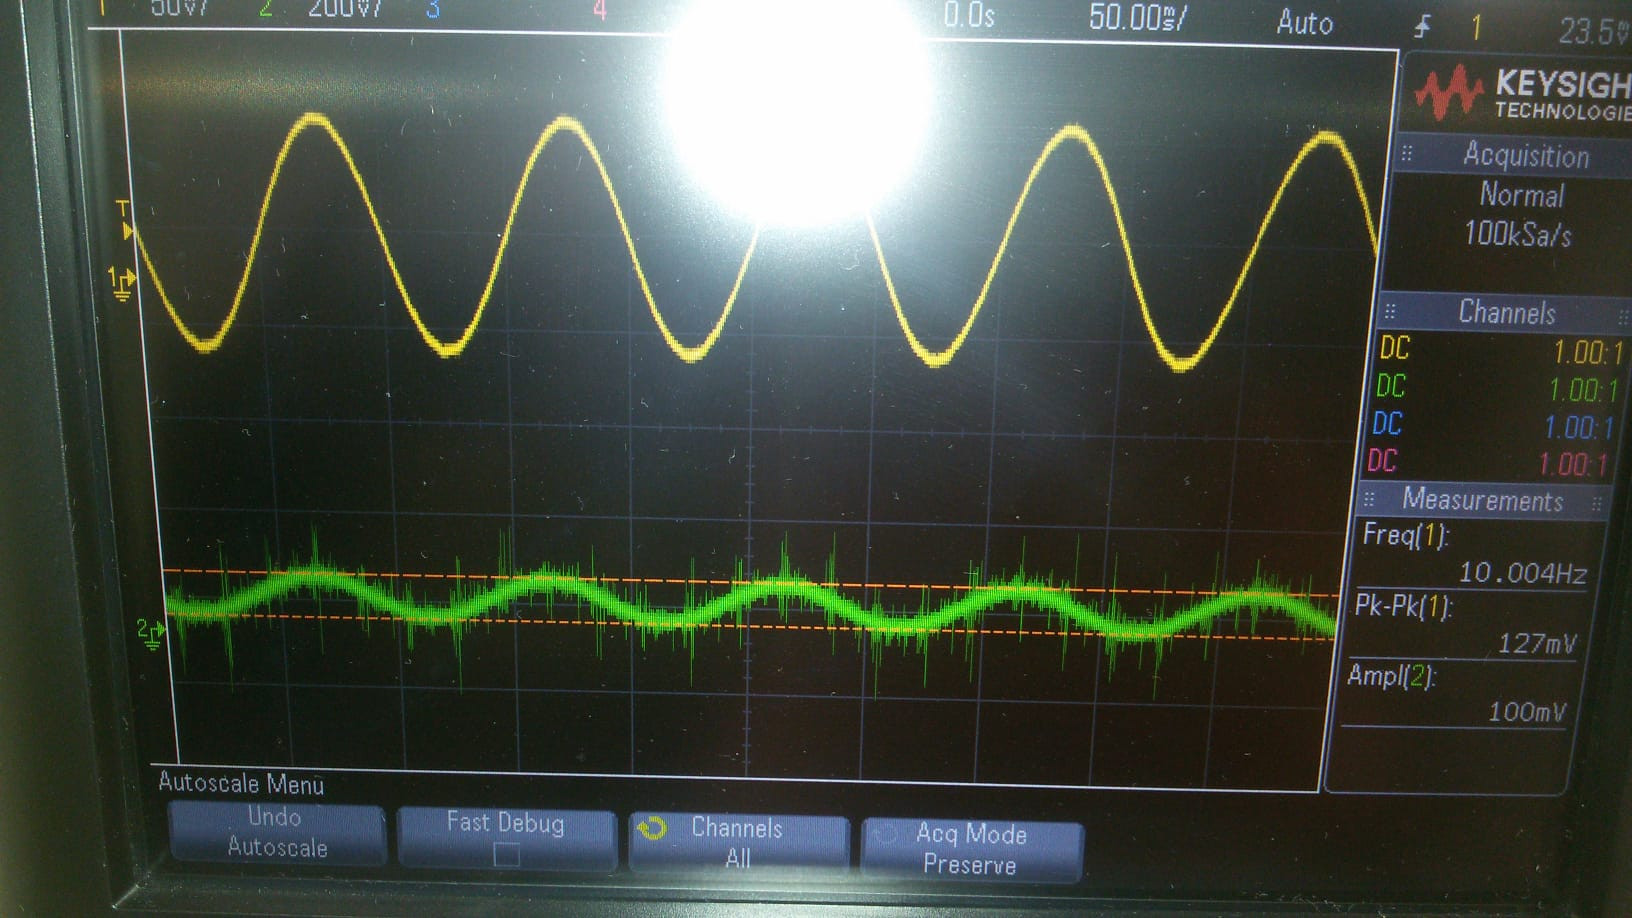
\includegraphics[width=0.6\linewidth]{10Hz.jpeg}
\caption{The voltage of the laboratory test for a frequency of $10Hz$.}
\label{Fig9: 10Hz}
\end{figure}

\begin{figure}[H] 
\centering
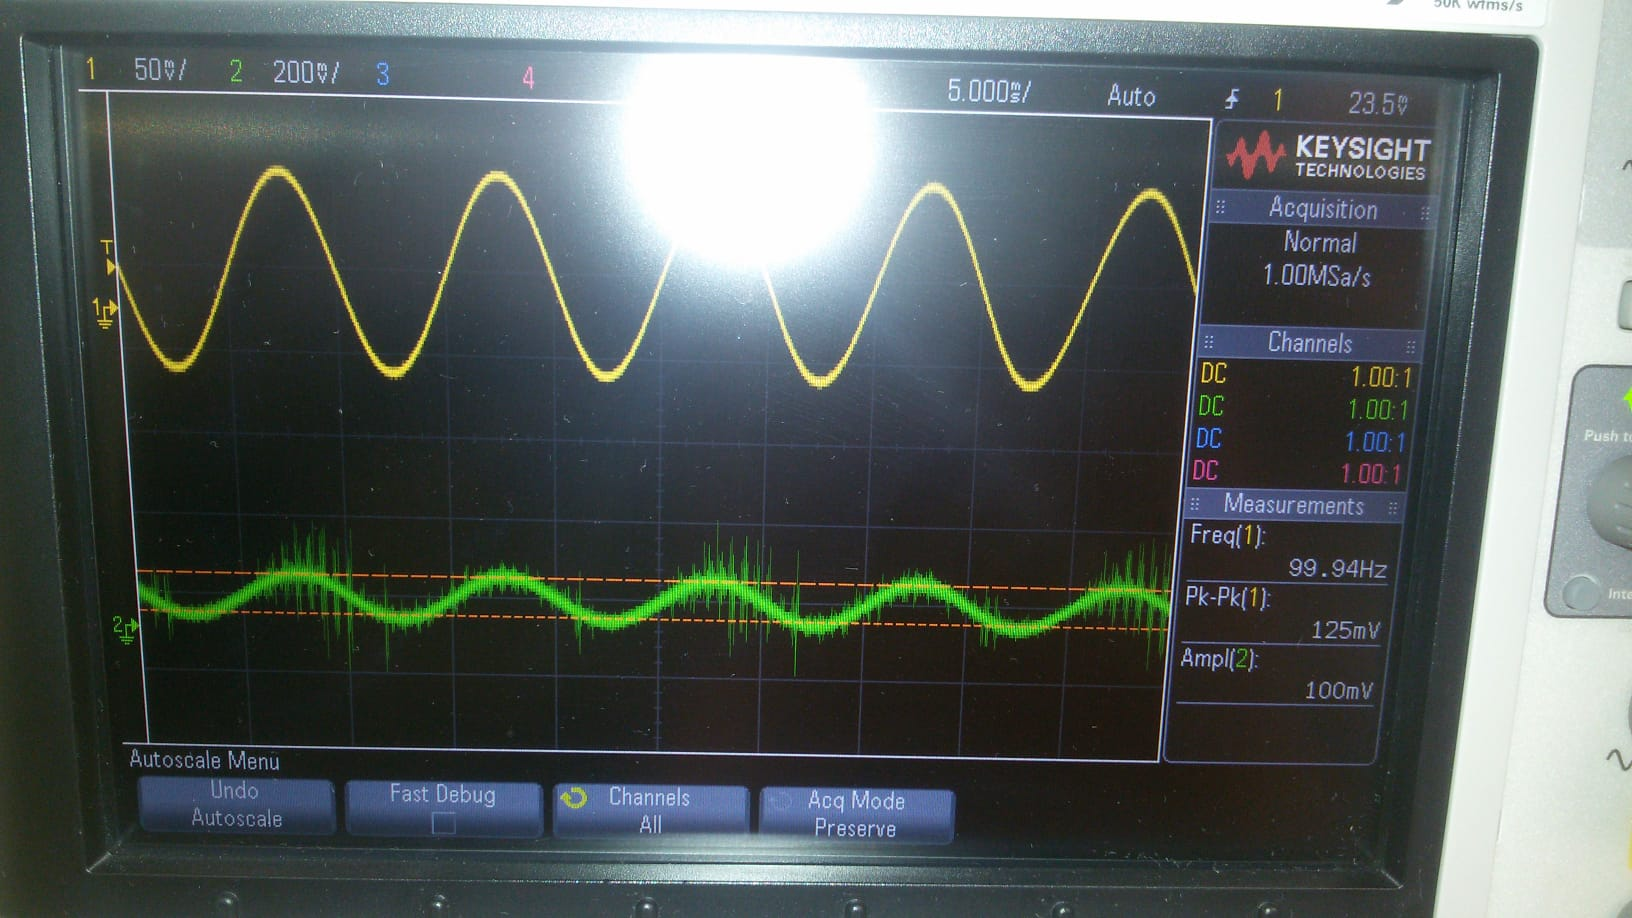
\includegraphics[width=0.6\linewidth]{100Hz.jpeg}
\caption{The voltage of the laboratory test for a frequency of $100Hz$.}
\label{Fig10: 100Hz}
\end{figure}

\begin{figure}[H] 
\centering
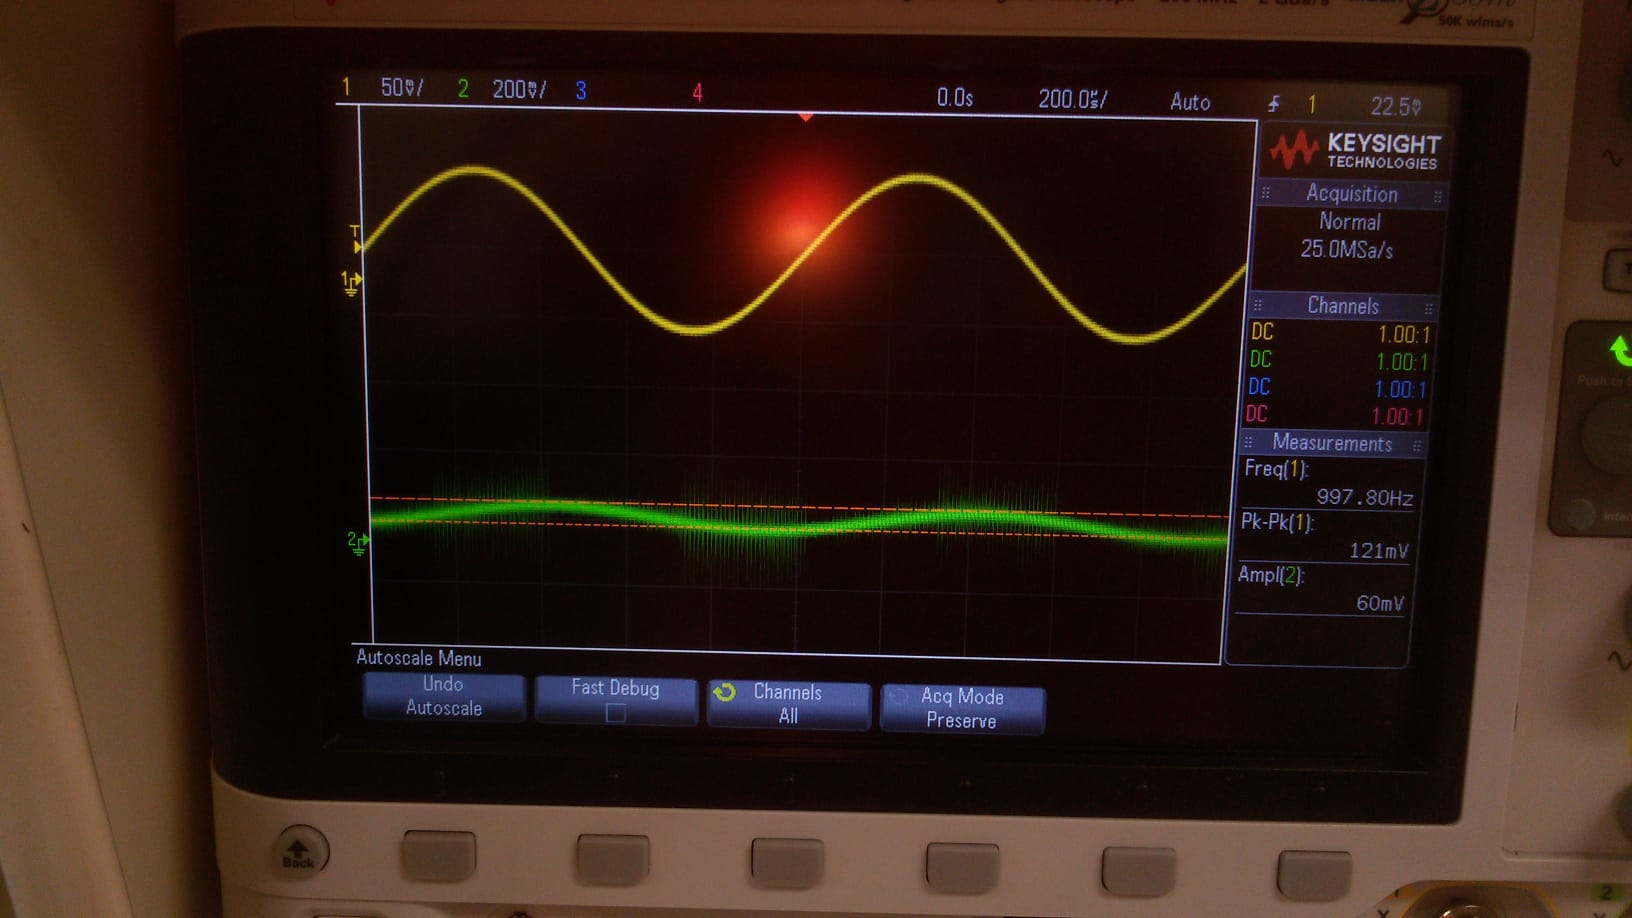
\includegraphics[width=0.6\linewidth]{1000Hz.jpeg}
\caption{The voltage of the laboratory test for a frequency of $1000Hz$.}
\label{Fig11: 1000Hz}
\end{figure}
